\documentclass[11pt]{article}
\usepackage[a4paper,margin=23mm]{geometry}
\usepackage[T1]{fontenc}
\usepackage{helvet}
\usepackage{xcolor}
\usepackage{booktabs}
\usepackage{longtable}
\usepackage{array}
\usepackage{graphicx}
\usepackage{pdfpages}
\usepackage{pdflscape}
\usepackage{xurl}
\usepackage{seqsplit}
\usepackage{hyperref}
\usepackage{microtype}
\renewcommand{\familydefault}{\sfdefault}
\definecolor{ink}{HTML}{17324D}
\definecolor{accent}{HTML}{D55E00}
\color{ink}
\hypersetup{colorlinks=true,linkcolor=accent,urlcolor=accent,citecolor=accent}
\setlength{\parindent}{0pt}
\setlength{\parskip}{5pt}
\newcommand{\hash}[1]{{\small\ttfamily\seqsplit{#1}}}
\newcommand{\PrimaryMetricRows}{%
GloVe target & 1.0000 & 0.5000 & [0.4639, 0.5392] & 0.3333 & 0.5000 & 1.0000 & 0.5000 \\
GloVe context ($\pm 2$) & 0.6506 & 0.5549 & [0.5156, 0.5956] & 0.5511 & 0.5670 & 0.4639 & 0.5800 \\
BERT mean last four & 0.5813 & 0.6708 & [0.6364, 0.7085] & 0.6673 & 0.6416 & 0.7743 & 0.7163 \\}
\newcommand{\LayerMetricRows}{%
1 & 0.8546 & 0.5705 & 0.5685 & 0.5900 \\
2 & 0.8145 & 0.6019 & 0.6014 & 0.6187 \\
3 & 0.7590 & 0.6113 & 0.6113 & 0.6357 \\
4 & 0.7330 & 0.6317 & 0.6314 & 0.6575 \\
5 & 0.6949 & 0.6458 & 0.6451 & 0.6768 \\
6 & 0.6564 & 0.6442 & 0.6419 & 0.6853 \\
7 & 0.6299 & 0.6489 & 0.6467 & 0.6946 \\
8 & 0.6039 & 0.6599 & 0.6558 & 0.7036 \\
9 & 0.5728 & 0.6661 & 0.6624 & 0.7093 \\
10 & 0.5625 & 0.6599 & 0.6543 & 0.7197 \\
11 & 0.5947 & 0.6536 & 0.6508 & 0.7096 \\
12 & 0.4942 & 0.6364 & 0.6308 & 0.6971 \\}
\newcommand{\SelectionRows}{%
Static context & glove\_context\_2 & 0.5840 & 0.5961 & yes \\
Static context & glove\_context\_5 & 0.5883 & 0.5928 & no \\
Static context & glove\_context\_10 & 0.5917 & 0.5863 & no \\
Static context & glove\_context\_sentence & 0.5930 & 0.5845 & no \\
BERT & layer\_12 & 0.6789 & 0.7145 & no \\
BERT & mean\_last\_four & 0.6891 & 0.7247 & yes \\}
\newcommand{\PairedRows}{%
Target GloVe minus nearby GloVe & Accuracy & -0.0549 & [-0.1176, 0.0094] \\
Target GloVe minus nearby GloVe & Macro F1 & -0.2178 & [-0.2661, -0.1710] \\
Target GloVe minus nearby GloVe & ROC-AUC & -0.0800 & [-0.1273, -0.0378] \\
Target GloVe minus BERT & Accuracy & -0.1708 & [-0.2195, -0.1238] \\
Target GloVe minus BERT & Macro F1 & -0.3340 & [-0.3739, -0.2953] \\
Target GloVe minus BERT & ROC-AUC & -0.2163 & [-0.2588, -0.1775] \\
Nearby GloVe minus BERT & Accuracy & -0.1160 & [-0.1693, -0.0658] \\
Nearby GloVe minus BERT & Macro F1 & -0.1161 & [-0.1690, -0.0664] \\
Nearby GloVe minus BERT & ROC-AUC & -0.1363 & [-0.1912, -0.0811] \\}

\title{Static vs Contextual Embeddings for Lexical Ambiguity:\\
A Word-in-Context Evaluation\\Method and Results Appendix}
\author{Choudhary Prashant Santosh (1910474) \and Rahul Khunt (1911272)}
\date{September 2026}
\begin{document}
\maketitle
\tableofcontents

\noindent\textbf{Project repository:} \url{https://github.com/Mr-Dark-debug/static-contextual-ambiguity}

\section{Research question and scope}
This project asks whether a context-sensitive target representation distinguishes
same-sense from different-sense uses more effectively than static alternatives.
It compares type-level GloVe, a lexical GloVe context mean, and an unfine-tuned
BERT-base target representation. It is a controlled representation probe, not a
claim about fine-tuned task state of the art.

\section{Dataset provenance and audit}
The source is the official SuperGLUE v2 WiC archive at
\url{https://dl.fbaipublicfiles.com/glue/superglue/data/v2/WiC.zip}. Its SHA-256 is
\hash{ee7e67f4ae9eafbf533780faa198e62167f3cda54256cdf261877be3c0e90900}.
The release is distributed under CC BY-NC 4.0 by the WiC authors.

\begin{table}[h]
\centering
\caption{Validated release counts and span diagnostics.}
\begin{tabular}{lrrrrrr}
\toprule
Split & Rows & Positive & Negative & Unlabeled & Lemma mismatch & Repeated surface \\
\midrule
Train & 5,428 & 2,714 & 2,714 & 0 & 1,852 & 93 \\
Validation & 638 & 319 & 319 & 0 & 251 & 1 \\
Test & 1,400 & 0 & 0 & 1,400 & 521 & 20 \\
\bottomrule
\end{tabular}
\end{table}

All target spans are non-empty half-open character intervals. IDs are unique
within splits. Four symmetric duplicate pairs occur within training, none within
validation, and no task pair crosses train and validation. The label-hidden test
split is audited but not evaluated.

\section{Representations}
\subsection{Static baselines}
GloVe uses the 6B-token, uncased, 300-dimensional release. Archive SHA-256:
\hash{617afb2fe6cbd085c235baf7a465b96f4112bd7f7ccb2b2cbd649fed9cbcf2fb}.
The target diagnostic looks up the supplied lemma on both sides, making every
available paired cosine exactly 1 by construction. Eighteen training lemmas are
OOV; missing target scores are replaced by the median finite training score.

Context vectors average in-vocabulary regex word tokens after excluding only the
token span that overlaps the marked target. Candidate windows are $\pm2$,
$\pm5$, $\pm10$, and the sentence. If a context side has no usable token, it falls
back to that side's target lemma; this occurs once per window in training and zero
times in validation. No evaluated context pair remains missing.

\subsection{Contextual target}
The encoder is \path{google-bert/bert-base-uncased}, revision
\hash{f584a14f45f850d60d0036d54f3e4dfdb3d52075}. It remains in evaluation mode;
there is no fine-tuning. A fast tokenizer emits character offsets. Every
WordPiece satisfying \texttt{token\_end > target\_start} and
\texttt{token\_start < target\_end} is selected, ignoring zero-width special
tokens, and selected WordPieces are averaged. Layers 1-12 and mean-last-four are
cached from one forward pass.

\section{Selection and evaluation protocol}
The balanced training labels are stratified into 4,342 tune and 1,086 internal
holdout rows using seed 2026. Candidate thresholds are fitted on tune rows by
macro F1. Candidate representations are ranked on internal-holdout macro F1,
then accuracy, ROC-AUC, and declared simplicity order. Winners are frozen before
validation metrics are computed. Thresholds are then refitted on all 5,428
training rows. Selection ledger hash:
\hash{debfd61b068f22ea1a737f238bd90ea4fb8bf44f675907e428949b559a0bb309}.

\begin{longtable}{llrrc}
\caption{Training-only candidate selection.}\\
\toprule
Family & Candidate & Tune macro F1 & Holdout macro F1 & Selected \\
\midrule
\endfirsthead
\toprule
Family & Candidate & Tune macro F1 & Holdout macro F1 & Selected \\
\midrule
\endhead
\SelectionRows
\bottomrule
\end{longtable}

\section{Primary validation results}
Predictions use score $\geq$ threshold as same-sense. Precision and recall use
same-sense as the positive label. Confusion-matrix layout is TN, FP / FN, TP.
Intervals are percentile intervals from 1,000 fixed-seed paired example
resamples.

\begin{landscape}
\begin{longtable}{lrrrrrrr}
\caption{Primary results on 638 balanced validation pairs.}\\
\toprule
System & Threshold & Accuracy & Accuracy 95\% CI & Macro F1 & Precision & Recall & ROC-AUC \\
\midrule
\endfirsthead
\toprule
System & Threshold & Accuracy & Accuracy 95\% CI & Macro F1 & Precision & Recall & ROC-AUC \\
\midrule
\endhead
\PrimaryMetricRows
\bottomrule
\end{longtable}
\end{landscape}

The selected BERT representation is correct on 428 pairs; GloVe context is
correct on 354. BERT alone is correct on 178 pairs, GloVe context alone on 104,
both on 250, and both primary systems are wrong on 106.

\begin{longtable}{llrr}
\caption{Paired primary-system differences with 95\% intervals.}\\
\toprule
Contrast & Metric & Estimate & 95\% interval \\
\midrule
\endfirsthead
\toprule
Contrast & Metric & Estimate & 95\% interval \\
\midrule
\endhead
\PairedRows
\bottomrule
\end{longtable}

The accuracy, macro-F1, and ROC-AUC intervals for GloVe context minus BERT all
exclude zero. This supports a difference under the current paired sample and
protocol; it does not provide a universal model ordering.

\section{Secondary BERT layer analysis}
Each layer threshold is trained on all training pairs. Validation layer results
are descriptive and do not replace the frozen primary representation.

\begin{table}[h]
\centering
\caption{Individual BERT target layers.}
\begin{tabular}{rrrrr}
\toprule
Layer & Threshold & Accuracy & Macro F1 & ROC-AUC \\
\midrule
\LayerMetricRows
\bottomrule
\end{tabular}
\end{table}

Accuracy rises broadly from layer 1 to layer 9 and then declines through layer
12. Layer 10 has the largest individual-layer ROC-AUC. This is compatible with
the train-selected mean-last-four result, but validation was not reused for
selection.

\section{Error analysis}
System-agreement partitions are disjoint. There are 250 both-primary-correct,
178 BERT-only-correct, 104 static-only-correct, 54 all-system-wrong, and 52 rows
where both primary systems are wrong but the one-class target diagnostic is
right. For BERT, error margin is absolute distance from the frozen cosine
threshold. Of 210 errors, 33 are within 0.025 and 53 occupy the top error-margin
quartile.

BERT recovers 77.43\% of same-sense pairs and 56.74\% of different-sense pairs;
GloVe context recovers 46.39\% and 64.58\%, respectively. These are descriptive
class skews. Saved high-margin examples include a same-sense anatomical
\emph{ball}/\emph{balls} pair that BERT separates strongly and different-sense
\emph{engrave} and \emph{map} pairs that it places close together. Conversely,
BERT links low-overlap same-sense examples such as \emph{rust remover}/\emph{paint
remover}. Fine sense granularity and constructional similarity are plausible
explanations, not causal findings.

\section{Reproducibility record}
The locked runtime is Python 3.11.15, NumPy 2.4.6, PyTorch 2.11.0+cu130, and
Transformers 5.17.0. Full inference ran on an NVIDIA GeForce RTX 3050 Ti Laptop
GPU. Arrays are keyed by dataset fingerprint, model revision, maximum length,
seed, and cache schema. The clean cached reproduction recorded Git commit
\texttt{7c6c956a173920b8aa685e206b9e4cdade1afdb6} on branch \texttt{main}.

\section{Limitations}
The sample covers one English benchmark; bootstrap intervals omit dataset-design
and modeling uncertainty. BERT is an older frozen base encoder. The static
context baseline has no syntax, weighting, subword model, or supervised
classifier. A global cosine threshold compresses potentially useful geometry.
Surface-mismatch groups are observational and confounded. No score is reported
for the label-hidden test split.

\section{Author contributions and use of AI tools}
\emph{AI-assisted wording notice: OpenAI Codex drafted the wording of this
section for the authors to verify before signing their declarations.}

The authors selected WiC, designed the three comparison conditions, initialized
the frozen GloVe and BERT checkpoints, and chose settings and thresholds using
training data only. They ran and checked the audit, inference, validation
analysis, tables, and figures. They did not train or fine-tune model weights.
The saved selection ledger, predictions, and metrics record these choices.

The authors chose the poster's explanations, examples, and graphs and checked
the numbers against saved results. Canva helped explore the layout; the final
poster was assembled in LaTeX. GLM assisted with LaTeX layout code. OpenAI
Codex provided limited coding suggestions and debugging in an interactive
paired-programming process. It also drafted this disclosure, revised appendix
wording and the poster's final italic sentence, and checked the PDFs. The
authors remain responsible for the code, claims, figures, and final submission.
No AI detector score is
used as evidence of authorship.

\section{References}
\begin{thebibliography}{99}
\bibitem{survey} J. Camacho-Collados and M. T. Pilehvar. From Word to Sense
Embeddings: A Survey on Vector Representations of Meaning. \emph{JAIR}, 2018.
\url{https://doi.org/10.1613/jair.1.11259}.
\bibitem{wic} M. T. Pilehvar and J. Camacho-Collados. WiC: The Word-in-Context
Dataset for Evaluating Context-Sensitive Meaning Representations. NAACL, 2019.
\url{https://doi.org/10.18653/v1/N19-1128}.
\bibitem{superglue} A. Wang et al. SuperGLUE: A Stickier Benchmark for
General-Purpose Language Understanding Systems. NeurIPS, 2019.
\url{https://papers.nips.cc/paper_files/paper/2019/hash/4496bf24afe7fab6f046bf4923da8de6-Abstract.html}.
\bibitem{glove} J. Pennington, R. Socher, and C. D. Manning. GloVe: Global Vectors
for Word Representation. EMNLP, 2014.
\url{https://doi.org/10.3115/v1/D14-1162}.
\bibitem{bert} J. Devlin, M.-W. Chang, K. Lee, and K. Toutanova. BERT:
Pre-training of Deep Bidirectional Transformers for Language Understanding.
NAACL, 2019. \url{https://doi.org/10.18653/v1/N19-1423}.
\bibitem{loureiro} D. Loureiro et al. Analysis and Evaluation of Language Models
for Word Sense Disambiguation. \emph{Computational Linguistics}, 2021.
\url{https://doi.org/10.1162/coli_a_00405}.
\bibitem{zhou} Y. Zhou and D. Bollegala. Learning Sense-Specific Static Embeddings
using Contextualised Word Embeddings as a Proxy. PACLIC, 2021.
\url{https://aclanthology.org/2021.paclic-1.53/}.
\bibitem{rawc} S. Trott and B. Bergen. RAW-C: Relatedness of Ambiguous Words in
Context. ACL-IJCNLP, 2021. \url{https://doi.org/10.18653/v1/2021.acl-long.550}.
\bibitem{haber} J. Haber and M. Poesio. Patterns of Polysemy and Homonymy in
Contextualised Language Models. Findings of EMNLP, 2021.
\url{https://doi.org/10.18653/v1/2021.findings-emnlp.226}.
\bibitem{soper} E. Soper and J.-P. Koenig. When Polysemy Matters: Modeling
Semantic Categorization with Word Embeddings. *SEM, 2022.
\url{https://doi.org/10.18653/v1/2022.starsem-1.10}.
\bibitem{fodor} J. Fodor, S. De Deyne, and S. Suzuki. The Importance of Context in
the Evaluation of Word Embeddings: The Effects of Antonymy and Polysemy. IWCS,
2023. \url{https://aclanthology.org/2023.iwcs-1.16/}.
\bibitem{erren} T. C. Erren and P. E. Bourne. Ten Simple Rules for a Good Poster
Presentation. \emph{PLOS Computational Biology}, 2007.
\url{https://doi.org/10.1371/journal.pcbi.0030102}.
\bibitem{wic_archive} SuperGLUE. WiC v2 dataset archive.
\url{https://dl.fbaipublicfiles.com/glue/superglue/data/v2/WiC.zip}.
\bibitem{glove_release} Stanford NLP. GloVe pretrained-vector release, 6B tokens,
300 dimensions. \url{https://nlp.stanford.edu/projects/glove/}.
\bibitem{bert_checkpoint} Google BERT. \texttt{bert-base-uncased} model card and
checkpoint. \url{https://huggingface.co/google-bert/bert-base-uncased}.
\end{thebibliography}

\clearpage
% One official form for each author. Replace both unsigned pages with a
% two-page PDF of the personally signed forms for the final submission.
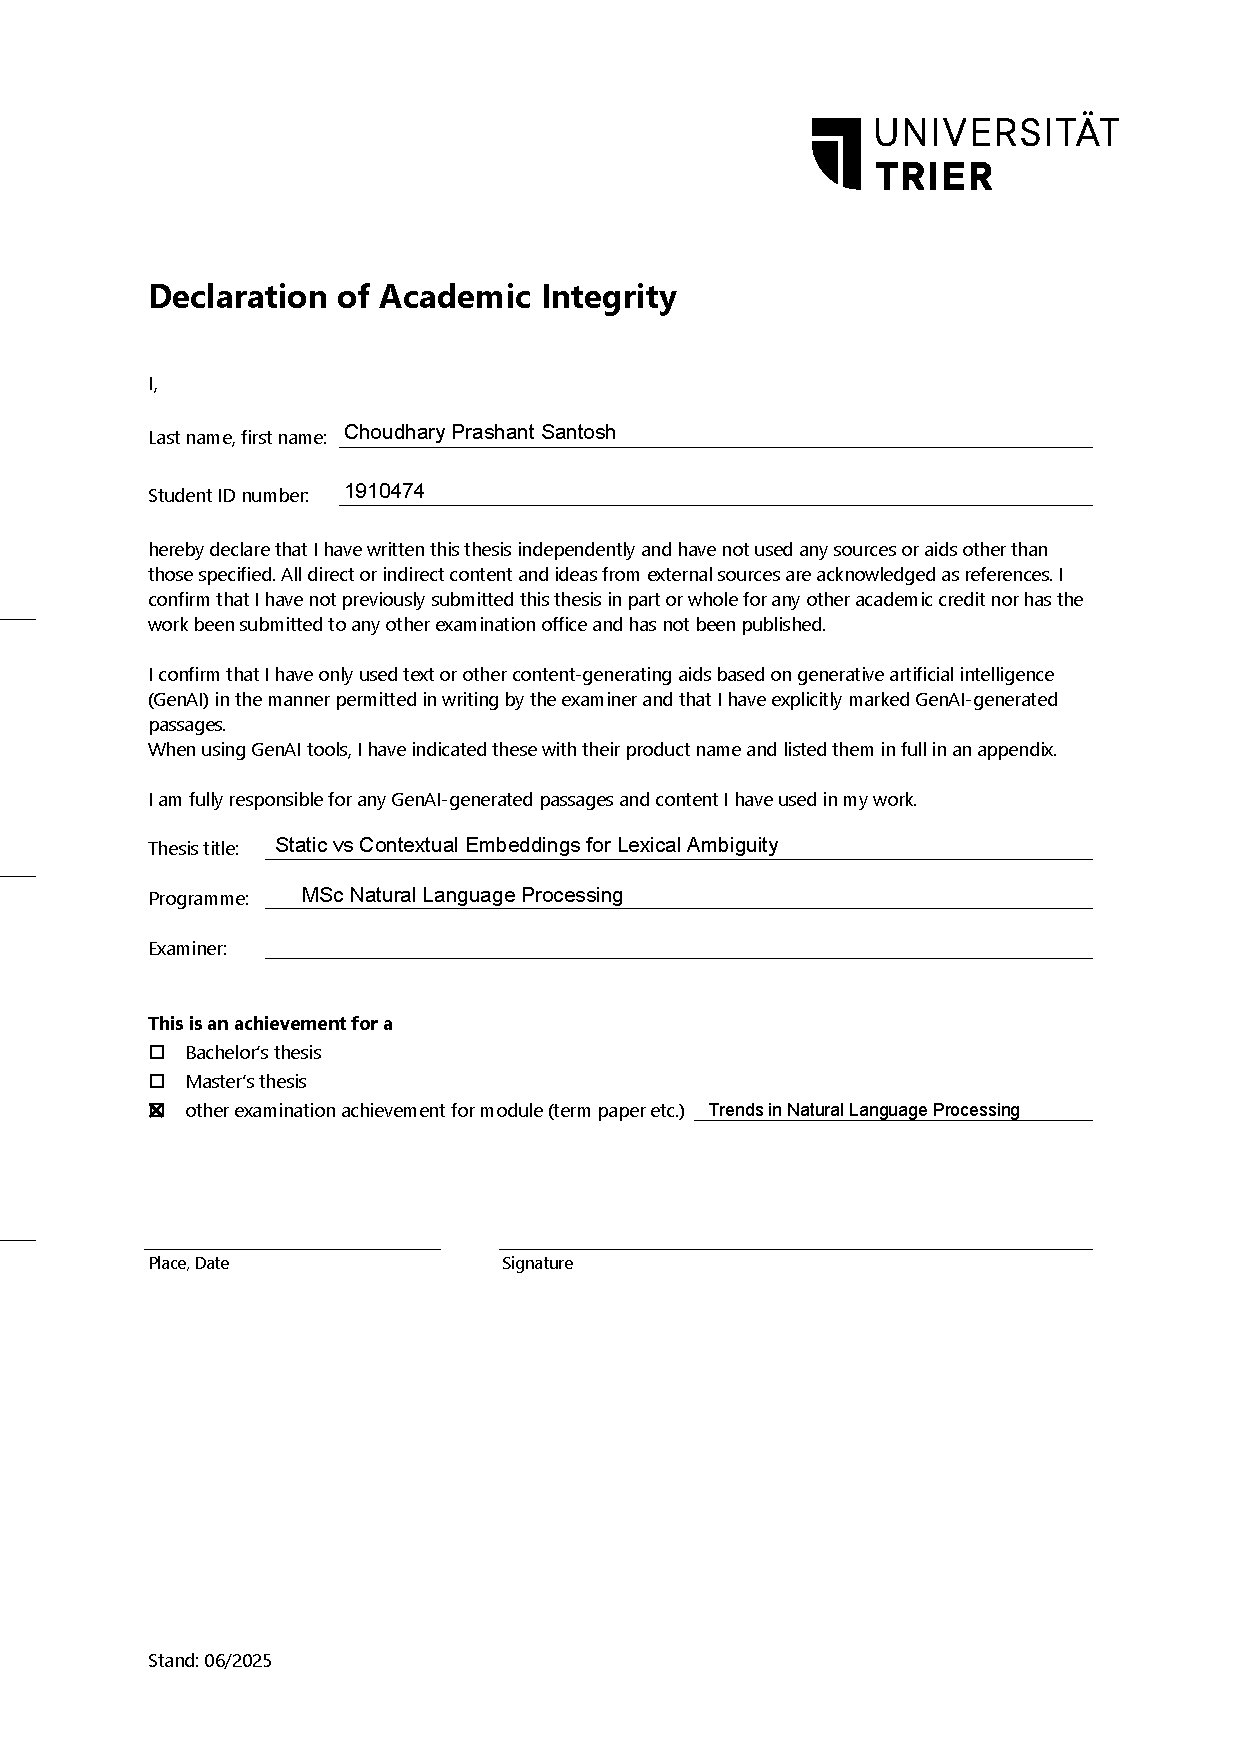
\includepdf[pages=-]{declaration_1910474_unsigned.pdf}
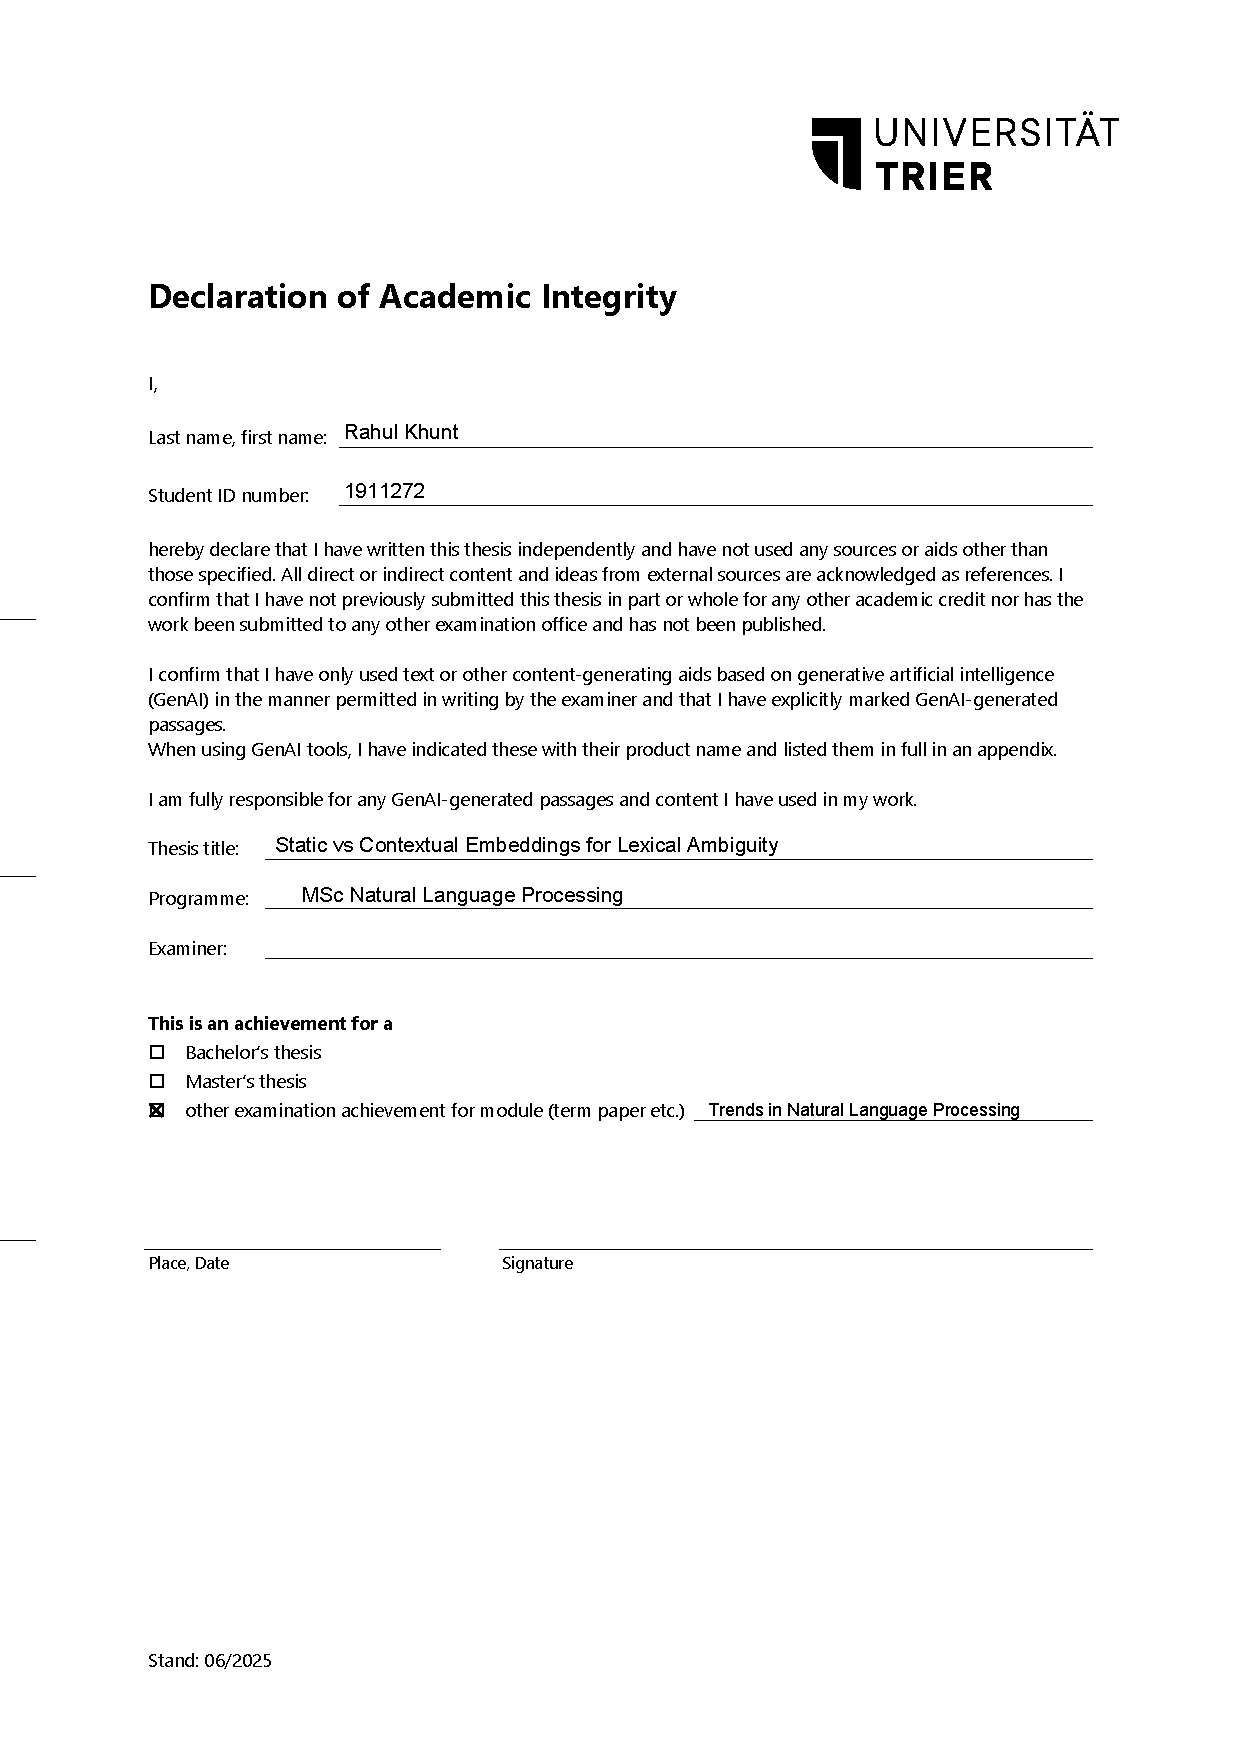
\includepdf[pages=-]{declaration_1911272_unsigned.pdf}
\end{document}
